\documentclass[12pt, a4paper, spanish, british, twoside]{article}
\usepackage[
  margin=3.2cm,
  includefoot,
  footskip=30pt
]{geometry}
\usepackage{authblk}
%Fonts
\usepackage[T1]{fontenc}
\usepackage[utf8]{inputenc}
\usepackage[11pt]{moresize}
\usepackage{anyfontsize}
\usepackage{textgreek}
%Figures
\usepackage{graphicx}
\usepackage{wrapfig}
\usepackage{floatrow}
\usepackage{subfig}
\captionsetup[figure]{font=small,labelfont=small}\usepackage{transparent}
\usepackage{eso-pic}
\usepackage{chngcntr}
\graphicspath{{./assets/}}
%Tables
\usepackage{tabu}
\usepackage{longtable}
\usepackage{multirow}
\usepackage{booktabs}
\usepackage{float}
\floatstyle{plaintop}
\restylefloat{table}
\renewcommand{\tablename}{Table}
\usepackage{color, colortbl}
%Maths
\usepackage{amsmath}
\usepackage{amssymb}
\usepackage{dsfont}
\usepackage{braket}
\usepackage{mathtools}
\usepackage{mhchem}
\usepackage{slashed}
\usepackage[makeroom]{cancel}
\usepackage{mathrsfs}
\usepackage{siunitx}

%Absolute value
\DeclarePairedDelimiter\abs{\lvert}{\rvert}

%Norm
\DeclarePairedDelimiter\norm{\lVert}{\rVert}
\makeatletter
\let\oldabs\abs
\def\abs{\@ifstar{\oldabs}{\oldabs*}}
%
\let\oldnorm\norm
\def\norm{\@ifstar{\oldnorm}{\oldnorm*}}
\makeatother


%Trace
\DeclarePairedDelimiter\tr{\text{Tr}\lbrace}{\rbrace}

%Commutator
\DeclarePairedDelimiterX\com[2]{[}{]}{#1 , #2}
%Anti-commutator
\DeclarePairedDelimiterX\acom[2]{\lbrace}{\rbrace}{#1 , #2}

%Dagger
\newcommand{\+}{\dagger}
%identity
\newcommand{\id}{\mathbbm{1}}
%partial
\newcommand{\del}{\partial}
%mute proof title
\newcommand{\mute}{\unskip\nopunct}
%differential d
\AtBeginDocument{\renewcommand{\d}{\text{d}}}

%Page Formatting
\usepackage[en-GB]{datetime2}
\DTMlangsetup[en-GB]{ord=omit}
\usepackage{fancyhdr}
\usepackage{afterpage}
\usepackage{titlesec}
\titlelabel{\thetitle.\quad}
\usepackage{blindtext}
\usepackage[bottom]{footmisc}
\renewcommand*\footnoterule{}
\renewcommand{\thefootnote}{\fnsymbol{footnote}}

%Chapter formatting
\usepackage{titlesec, blindtext, color}
\definecolor{gray75}{gray}{0.6}
\newcommand{\hsp}{\hspace{15pt}}

\titleformat{\chapter}[display]{\vspace*{-1cm}\centering\Huge\bfseries}{\vspace*{-2em}\fontsize{100}{110}\selectfont \textcolor{gray75}{\thechapter}}{-5pt}{\vspace*{-1em}\centering\huge\bfseries\textsc}[ \vspace*{-1em}\textcolor{gray75}{\titlerule}\vspace*{-1.5em}]


\titleformat{\section}
  {\Large\bfseries}{\thesection.}{0.5em}{\vspace*{0em}}

\titleformat{\subsubsection}
  {\bfseries}{\thesubsubsection}{0em}{\vspace*{0em}}

\renewcommand\sectionmark[1]{\markright{\thesection\ #1}}
%Hyperlinks for sections
\usepackage[hidelinks]{hyperref}
\hypersetup{
    allcolors=black
}

%Blank Page
\newcommand\blankpage{%
    \null
    \thispagestyle{empty}%
    \newpage}
    
%Double sided header and footer
\setlength{\headheight}{15pt}
\pagestyle{fancy}
\fancyhf{}
\fancyhead[LE,RO]{FYSS6320}
\fancyhead[RE,LO]{\textsc{Jorge Romero}}
\fancyfoot[RO,LE]{\thepage}
\renewcommand{\footrulewidth}{1pt}

% Redefine the plain page style
\fancypagestyle{plain}{
  \fancyhf{}%
  \fancyfoot[RO,LE]{\thepage}
  \renewcommand{\headrulewidth}{0pt}% Line at the header invisible
  \renewcommand{\footrulewidth}{1pt}}% Line at the footer visible

%Spacing for paragraphs and titles
\setlength{\parskip}{0.5em}
\titlespacing\section{0pt}{3pt}{0pt}\relax
\titlespacing\subsection{0pt}{12pt plus 4pt minus 2pt}{-\parskip}\relax
\titlespacing\subsubsection{0pt}{12pt plus 4pt minus 2pt}{-\parskip}\relax
%Code
\usepackage{color, soul}
\usepackage{xcolor}
\usepackage{listings}

\definecolor{mBlue}{rgb}{0,0,0.6}
\definecolor{mGray}{rgb}{0.2,0.2,0.2}
\definecolor{mRed}{rgb}{0.6,0,0}
\definecolor{backgroundColour}{rgb}{0.92,0.92,0.92}

\lstdefinestyle{CStyle}{
    backgroundcolor=\color{backgroundColour},   
    commentstyle=\color{mBlue},
    keywordstyle=\color{mRed},
    numberstyle=\tiny\color{mGray},
    stringstyle=\color{magenta},
    basicstyle=\footnotesize,
    breakatwhitespace=false,         
    breaklines=true,                 
    captionpos=b,                    
    keepspaces=true,                 
    numbers=left,                    
    numbersep=5pt,                  
    showspaces=false,                
    showstringspaces=false,
    showtabs=false,                  
    tabsize=2,
    language=C
}

%Autoref labels
\renewcommand{\figureautorefname}{Fig.}
\renewcommand{\tableautorefname}{Table}
\renewcommand{\tablename}{Table}
\renewcommand{\sectionautorefname}{Sec.}
\renewcommand{\subsectionautorefname}{Sec.}
\renewcommand{\appendixautorefname}{Appendix}
\renewcommand{\contentsname}{Contents}

\begin{document}

\begin{titlepage}
	
    \begin{center}
        
        \LARGE{\textbf{FYSS3550}}\\
        \large{\textbf{Techniques for Nuclear and Accelerator-based Physics Experiments}}\\
        \vspace{0.15\textheight}
        \LARGE{\textbf{Home Exam}}\\
        \vspace{0.05\textheight}
        \large{\textbf{19.04.2021-30.04.2021}}\\
    \end{center}
    \vspace{0.08\textheight}
    \begin{center}
       \large{\textbf{Jorge Romero}}\\\large{\textbf{joromero@jyu.fi}}
    \end{center}
    \vspace{0.05\textheight}
    \centering

        \large{\textbf{Department of Physics}}\\
    \centering
    \vfill
    
\includegraphics[width=0.5\textwidth]{jyu-keskitetty-kaksikielinen.eps}

\end{titlepage}

\pagenumbering{arabic}
\section{Introduction}
\label{sec:intro}
The Low Energy Branch (LEB) is a new facility, designed as an extension for the MARA (Mass Analysing Recoil Apparatus) deflector at the Accelerator Laboratory in the University of Jyväskylä.

MARA-LEB will serve as a system for additional isotopic and mass selection after MARA. One of MARA-LEB's most important components is its buffer gas cell. Within it, a noble gas (He or Ar) will flow at $\sim$500-1000\,mbar, which will stop and neutralise recoils coming from MARA at high charge states. The recoils will then be laser ionised and then transported to detectors via acceleration with radio-frequency quadrupoles (RFQ) and transport by electrodes, as shown in \autoref{fig:LEB_dia}, effectively selecting only one particular element from all recoils from MARA. A magnetic dipole will perform additional mass separation before the detector station for further purification of the beam.

\begin{figure}[H]
    \centering
    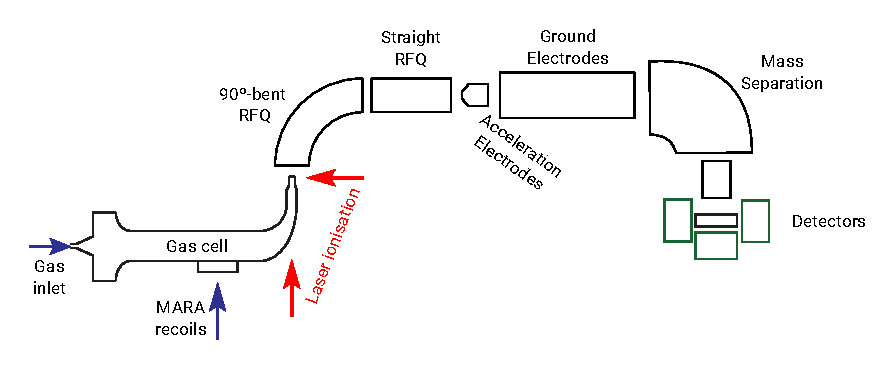
\includegraphics[width=\textwidth]{LEB.pdf}    
    \caption{Diagram of the MARA-LEB facility, highlighting the gas cell and showing in-gas-cell laser ionisation.}
    \label{fig:LEB_dia}
\end{figure}

The transport electrodes and mass separator have to be operated in vacuum, due to the use of strong electromagnetic fields that may discharge. However, the ions exiting the gas cell do so within a gas jet at relatively high pressures. Since this introduction of gas into the system is vital to the operation of MARA-LEB, but components down the beamline have to work in high vacuum, a system of {differential pumping} was designed for this facility. 

In this report, both the normal and differential pumping regions will be discussed, with special focus on the latter, due to its higher complexity. 
\newpage

\section{High Vacuum at MARA}
\label{sec:mara}
The first component of the LEB facility is the gas cell, which, as previously stated, is kept at relatively high pressures of 500-1000\,mbar, alongside the chamber it will be installed within. The gas cell will be placed at the MARA focal plane, to receive the mass-separated recoils coming from the deflector. MARA, however, is kept at high vacuum, of about $10^{-7}$\,mbar. Therefore, there must be a barrier separating these two regions, which should be strong enough to withstand pressure differences of up to  $10^{10}$\,mbar but not stop recoils from entering the gas cell.

A thin gas cell window will be installed at the entrance of the gas cell, and supported by a honeycomb structure, to separate these regions. The material and thickness of the window can be varied on a case-to-case basis, but several options have been suggested and simulated, such as 13\,\textmu m-thick Mylar or 4.5\,\textmu m-thick Havar.

\section{Pumping system}
\label{sec:pump}

The planned vacuum system for the facility includes three types of pumps, three types of valves and three types of gauges. The whole vacuum diagram can be seen in \autoref{fig:fullsystem}, where the different vacuum chambers are shown with their planned pumps, valves and gauges.

The vacuum components for each chamber have been selected specifically for their target pressures, which will not all be the same due to the presence of the differential pumping section. The gas cell chamber, which will house the gas cell and the 90º-bent RFQ, is planned to have pressures ranging from 0.1 to 0.01\,mbar, which means that the gas inside will be in a viscous regime. The second chamber, with the straight RFQ, will hold pressures from $10^{-2}$ down to $10^{-6}$\,mbar, having gas at an intermediate to molecular regime within it. The rest of the chambers (including the extraction chamber), will be maintained at a target pressure of $10^{-6}$\,mbar, at a molecular regime. 

\begin{figure}[h]
    \centering
    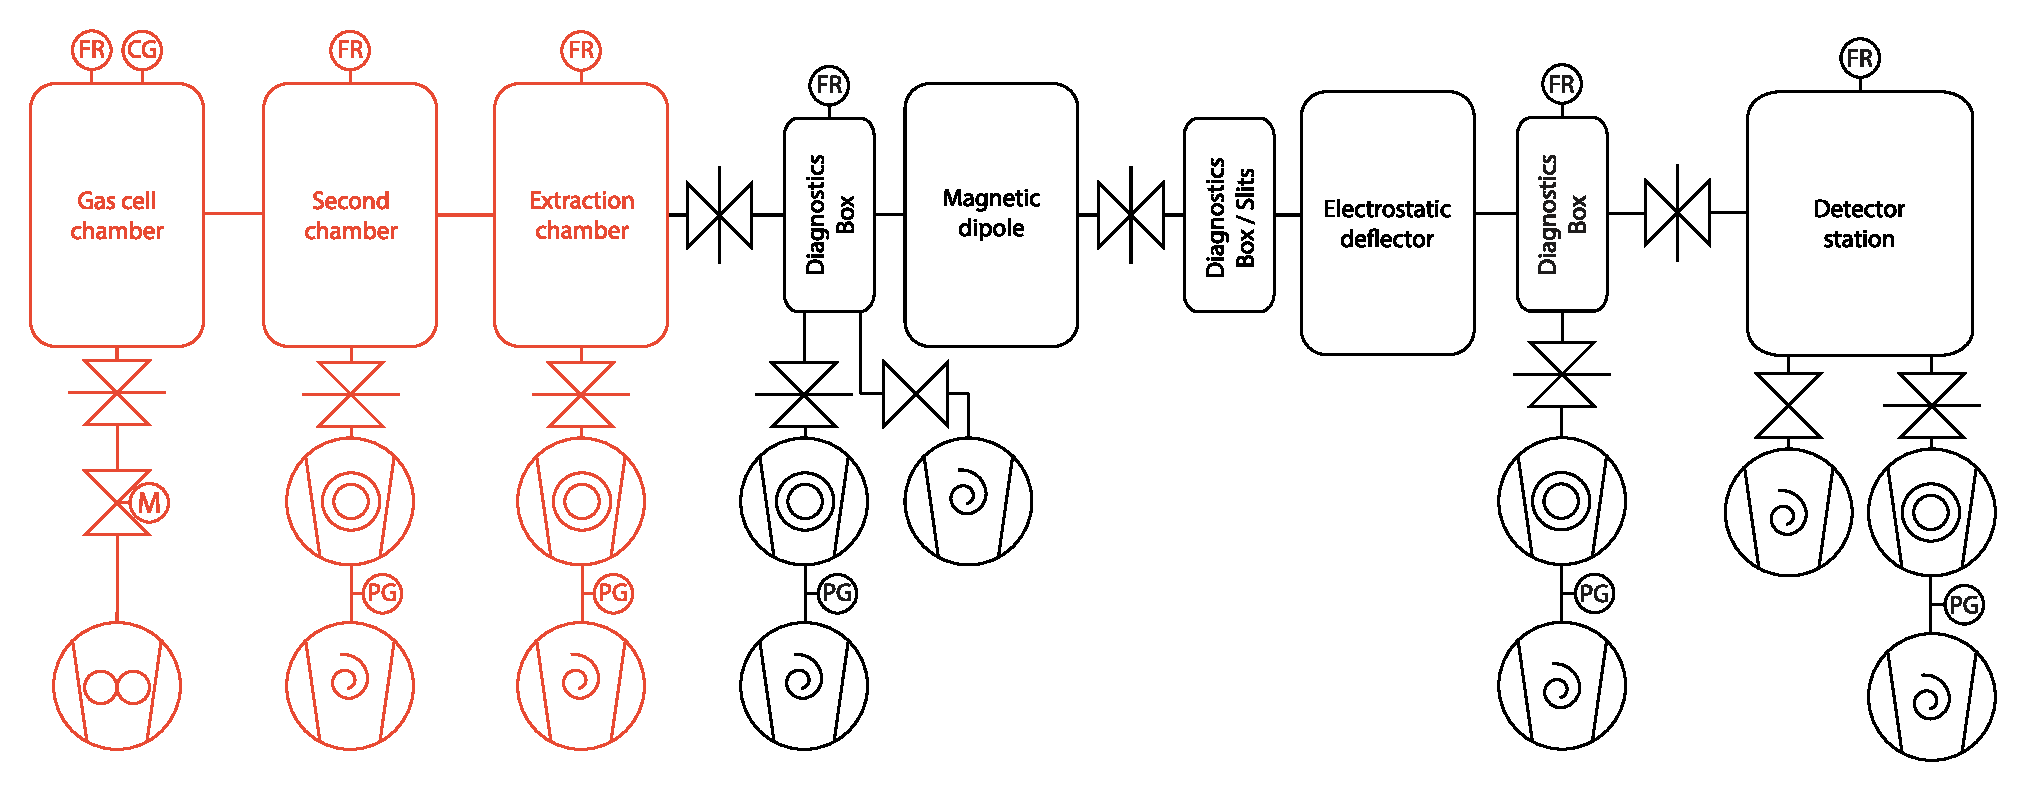
\includegraphics[width=1\textwidth]{pumpdia2.pdf}
     \caption{Full vacuum system diagram for the MARA-LEB facility, including pumps, gates and gauges to be used. The differential pumping region is highlighted in orange. The inset shows a legend for the diagram.}
     \label{fig:fullsystem}
 \end{figure}

\subsection{Pumps}
Every vacuum chamber, except the gas cell chamber, is pumped down by a turbomolecular (turbo) pump, with pumping speeds between 1000 and 2000\,L/s. These pumps are suited for molecular and intermediate regimes, which will be maintained in the chambers after an initial pumpdown.

Every turbo pump is backed by at least one  scroll pump; some chambers feature  two scroll pumps. These pumps are ideal for viscous flow, and will perform pumpdowns from ambient pressure. 

\begin{table}[h!]
    \caption{Different types of pumps planned for use in the MARA-LEB facility.}
     \label{tab:Pumps}
    \centering
    \hspace*{-0.5em}
    \begin{tabular}{@{}llll@{}}
    \hline
    \multicolumn{1}{c}{\textbf{Pump}} & \multicolumn{1}{c}{\textbf{Pump}}  & \multicolumn{1}{c}{\textbf{Pump}} & \multicolumn{1}{c}{\textbf{Pumping}} \\
    \multicolumn{1}{c}{\textbf{Location}} & \multicolumn{1}{c}{\textbf{Type}} & \multicolumn{1}{c}{\textbf{Model}} & {\textbf{Speed [L/s]}} \\
    \hline
    Gas Cell Chamber    & Screw     & GXS750/4200   & 960   \\ 
                                                            \\
    Second Chamber      & Turbo     & STP-iXR2206   & 2200  \\
                        & Scroll    & XDS35i        & 10    \\ 
                                                            \\
    Extraction Chamber  & Turbo     & STP-iXR1606   & 1000  \\
                        & Scroll    & XDS35i        & 10    \\
                                                            \\
    Diagnostics Box 1   & Turbo     & nEXT400D      & 400   \\
                        & Scroll    & nXDS6i        & 1.7   \\
                        & Scroll    & nXDS15i       & 5     \\
                                                            \\
    Diagnostics Box 2   & Turbo     & nEXT400D      & 400   \\
                        & Scroll    & nXDS6i        & 1.7   \\
                                                            \\
    Detector Station    & Turbo     & nEXT400D      & 400   \\
                        & Scroll    & nXDS6i        & 1.7   \\
                        & Scroll    & nXDS15i       & 5     \\
    \hline
    \end{tabular}
 \end{table}

\end{document}

